\documentclass[mathNotesPreamble]{subfiles}
\begin{document}
%\relscale{1.4}

\section{3.8: Implicit Differentiation}
Up until now, we have only taken the derivatives of \textit{explicitly} defined functions (functions defined in terms of only $x$). 

\noindent
An \textit{implicitly} defined function will be written in terms of both $x$ and $y$:
  $$x^2+y^2=25$$
\begin{center}
  \begin{tikzpicture}
    \begin{groupplot}[
      group style={group size=2 by 1},
      axis equal,
      axis lines=center,
      axis line style={->},
      ymin=-6.5, ymax=6.5,
      xtick={-5,5},
      ytick={-5,5},
      ticklabel style={font=\large, inner sep=0.75pt,fill=white},
      every axis plot/.append style={line width=0.95pt}, 
      samples=251, domain=-5:5,
      ]
      \nextgroupplot
        \addplot[-] expression[black]{sqrt(25-x^2)} node at (4.45,5.8) {$x^2+y^2=25$};
        \addplot[-] expression[black]{-sqrt(25-x^2)};
      \nextgroupplot
        \addplot[-] expression[ClemsonPurple]{sqrt(25-x^2)} node[black] at (4.1,5.8) {$y=\sqrt{25-x^2}$};
        \addplot[-] expression[ClemsonOrange]{-sqrt(25-x^2)} node[black] at (4.1,-5.5) {$y=-\sqrt{25-x^2}$};
    \end{groupplot}
  \end{tikzpicture}
\vfill 
  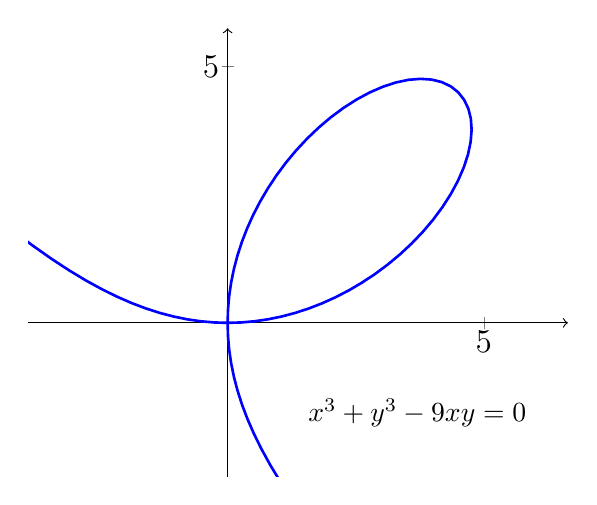
\begin{tikzpicture}
    \begin{axis}[
      axis equal,
      axis lines=center,
      axis line style={->},
      xmin=-3, xmax=5.75,
      ymin=-3, ymax=5.75,
      xtick={-5,5},
      ytick={-5,5},
      ticklabel style={font=\large, inner sep=0.75pt,fill=white},
      ]
      \draw[samples=100,domain=125:-40, line width=0.95pt, blue] plot(\x:{9*sin(\x)*cos(\x)/(sin(\x)^3+cos(\x)^3)}) node[black] at (3.7,-1.75) {$x^3+y^3-9xy=0$};
    \end{axis}
  \end{tikzpicture}
\vfill 
\end{center}
\pagebreak

\begin{center}\fbox{\parbox{0.7\linewidth}{

\textbf{Implicit Differentiation:}
  \begin{enumerate}
    \item Differentiate both sides of the equation with respect to $x$, treating $y$ as a differentiable function of $x$.
    \item Collect the terms with $\sfrac{dy}{dx}$ on one side of the equation.
    \item Solve for $\sfrac{dy}{dx}$.
  \end{enumerate}
}}\end{center}

\begin{ex*}
  Find the derivatives of the following by rewriting each function explicitly before taking the derivative, and by using implicit differentiation. Compare the results.
\end{ex*}

\begin{enumerate}[label=, itemsep=\stretch{1}]
  \item $y^2=x$
  \item $\sqrt x+\sqrt y=4$
\end{enumerate}
\vfill 
\pagebreak
\begin{ex*}
  Find the derivatives of the following equations:
\end{ex*}

\begin{tasks}[after-item-skip=\stretch{1}, label=~](2)
  \task $x^2+y^2=25$
  \task $x^3+y^3-9xy=0$
  \task $2y=x^2+\sin y$
  \task $x^2y^2+x\sin y=4$
  \task $y^5+x^2y^3=1+x^4y$
  \task $1+x=\sin\parens{xy^2}$
\end{tasks}
\vfill
\pagebreak

\begin{ex*}
  Find the derivatives of the following equations:
\end{ex*}
\begin{tasks}[after-item-skip=\stretch{1}, label=~](2)
  \task $x^3-xy+y^3=1$
  \task $xe^y=x-y$
  \task $\dfrac{1}{x}+\dfrac{1}{y}=1$
  \task $x^2-2x^3y^4+y^2=30y$
  \task $\tan(xy)=x+y$
  \task $x^2=\dfrac{x-y}{x+y}$
\end{tasks}
\vfill
\pagebreak

\begin{ex*}
  Find the second derivative implicitly for the following equations:
\end{ex*}
\begin{tasks}[after-item-skip=\stretch{1}, label=~](1)
  \task $y^2-2x=1-2y$
  \task $xy=\cot(xy)$
  \task $x^3+y^3=1$
  \task $x=e^y$
\end{tasks}
\vfill
\pagebreak

\begin{ex*}
  Find the equation of all lines tangent to the curve $x+y^3-y=1$ at $x=1$.
\end{ex*}
\vfill
%% This royal PITA needs to be compiled using 
%% shell-escape since it uses gnuplot
%%%%% pdflatex -shell-escape impFunc.tex %%%%%
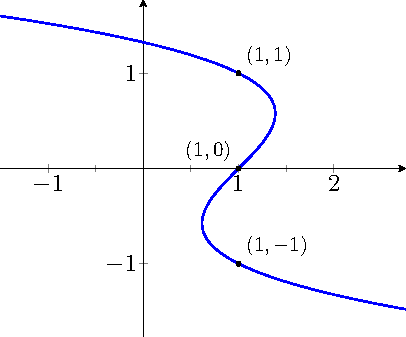
\includegraphics[width=0.4\linewidth]{impFunc1}

\begin{ex*}
  Find the equation of the tangent line and normal line for $\parens{x^2+y^2-2x}^2=2\parens{x^2+y^2}$ at $(x,y)=(2,2)$.  
\end{ex*}
\vfill
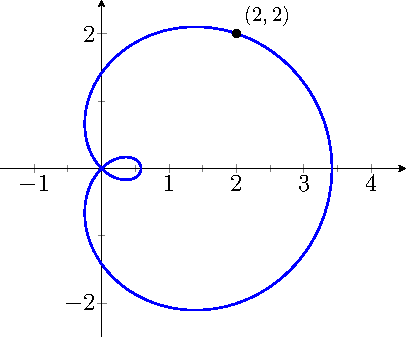
\includegraphics[width=0.4\linewidth]{impFunc2}

\pagebreak

\end{document}
